%package list
\documentclass{article}
\usepackage[top=3cm, bottom=3cm, outer=3cm, inner=3cm]{geometry}
\usepackage{multicol}
\usepackage{graphicx}
\usepackage{url}
%\usepackage{cite}
\usepackage{hyperref}
\usepackage{array}
%\usepackage{multicol}
\newcolumntype{x}[1]{>{\centering\arraybackslash\hspace{0pt}}p{#1}}
\usepackage{natbib}
\usepackage{pdfpages}
\usepackage{multirow}
\usepackage[normalem]{ulem}
\useunder{\uline}{\ul}{}
\usepackage{svg}
\usepackage{xcolor}
\usepackage{listings}
\lstdefinestyle{ascii-tree}{
    literate={├}{|}1 {─}{--}1 {└}{+}1 
  }
\lstset{basicstyle=\ttfamily,
  showstringspaces=false,
  commentstyle=\color{red},
  keywordstyle=\color{blue}
}
%\usepackage{booktabs}
\usepackage[labelformat=empty]{caption}
\usepackage{subcaption}
\usepackage{float}
\usepackage{array}

\newcolumntype{M}[1]{>{\centering\arraybackslash}m{#1}}
\newcolumntype{N}{@{}m{0pt}@{}}


%%%%%%%%%%%%%%%%%%%%%%%%%%%%%%%%%%%%%%%%%%%%%%%%%%%%%%%%%%%%%%%%%%%%%%%%%%%%
%%%%%%%%%%%%%%%%%%%%%%%%%%%%%%%%%%%%%%%%%%%%%%%%%%%%%%%%%%%%%%%%%%%%%%%%%%%%
\newcommand{\itemEmail}{cmestasz@unsa.edu.pe}
\newcommand{\itemStudent}{Christian Mestas Zegarra}
\newcommand{\itemCourse}{Fundamentos de la Programación 2}
\newcommand{\itemCourseCode}{1701213}
\newcommand{\itemSemester}{II}
\newcommand{\itemUniversity}{Universidad Nacional de San Agustín de Arequipa}
\newcommand{\itemFaculty}{Facultad de Ingeniería de Producción y Servicios}
\newcommand{\itemDepartment}{Departamento Académico de Ingeniería de Sistemas e Informática}
\newcommand{\itemSchool}{Escuela Profesional de Ingeniería de Sistemas}
\newcommand{\itemAcademic}{2023 - B}
\newcommand{\itemInput}{Del 11 Octubre 2023}
\newcommand{\itemOutput}{Al 16 Octubre 2023}
\newcommand{\itemPracticeNumber}{06}
\newcommand{\itemTheme}{ArrayList}
%%%%%%%%%%%%%%%%%%%%%%%%%%%%%%%%%%%%%%%%%%%%%%%%%%%%%%%%%%%%%%%%%%%%%%%%%%%%
%%%%%%%%%%%%%%%%%%%%%%%%%%%%%%%%%%%%%%%%%%%%%%%%%%%%%%%%%%%%%%%%%%%%%%%%%%%%

\usepackage[english,spanish]{babel}
\usepackage[utf8]{inputenc}
\AtBeginDocument{\selectlanguage{spanish}}
\renewcommand{\figurename}{Figura}
\renewcommand{\refname}{Referencias}
\renewcommand{\tablename}{Tabla} %esto no funciona cuando se usa babel
\AtBeginDocument{%
	\renewcommand\tablename{Tabla}
}

\usepackage{fancyhdr}
\pagestyle{fancy}
\fancyhf{}
\setlength{\headheight}{30pt}
\renewcommand{\headrulewidth}{1pt}
\renewcommand{\footrulewidth}{1pt}
\fancyhead[L]{\raisebox{-0.2\height}{
\includegraphics[width=3cm]{img/logo_episunsa.png}}}
\fancyhead[C]{\fontsize{7}{7}\selectfont	\itemUniversity \\ \itemFaculty \\ \itemDepartment \\ \itemSchool \\ \textbf{\itemCourse}}
\fancyhead[R]{\raisebox{-0.2\height}{
\includegraphics[width=1.2cm]{img/logo_abet}}}
\fancyfoot[L]{Christian Mestas}
\fancyfoot[C]{\itemCourse}
\fancyfoot[R]{Página \thepage}

% para el codigo fuente
\usepackage{listings}
\usepackage{color, colortbl}
\definecolor{dkgreen}{rgb}{0,0.6,0}
\definecolor{gray}{rgb}{0.5,0.5,0.5}
\definecolor{mauve}{rgb}{0.58,0,0.82}
\definecolor{codebackground}{rgb}{0.95, 0.95, 0.92}
\definecolor{tablebackground}{rgb}{0.8, 0, 0}

\lstset{frame=tb,
	language=bash,
	aboveskip=3mm,
	belowskip=3mm,
	showstringspaces=false,
	columns=flexible,
	basicstyle={\small\ttfamily},
	numbers=none,
	numberstyle=\tiny\color{gray},
	keywordstyle=\color{blue},
	commentstyle=\color{dkgreen},
	stringstyle=\color{mauve},
	breaklines=true,
	breakatwhitespace=true,
	tabsize=3,
	backgroundcolor= \color{codebackground},
}

\begin{document}

\vspace*{10px}

\begin{center}
	\fontsize{17}{17} \textbf{ Informe de Laboratorio \itemPracticeNumber}
\end{center}
\centerline{\textbf{\Large Tema: \itemTheme}}
%\vspace*{0.5cm}	

\begin{flushright}
	\begin{tabular}{|M{2.5cm}|N|}
		\hline
		\rowcolor{tablebackground}
		\color{white} \textbf{Nota} \\
		\hline
		\\[30pt]
		\hline
	\end{tabular}
\end{flushright}

\begin{table}[H]
	\begin{tabular}{|M{4.7cm}|M{4.8cm}|M{4.8cm}|}
		\hline
		\rowcolor{tablebackground}
		\color{white} \textbf{Estudiante} & \color{white}\textbf{Escuela} & \color{white}\textbf{Asignatura}                                        \\
		\hline
		{\itemStudent \par \itemEmail}    & \itemSchool                   & {\itemCourse \par Semestre: \itemSemester \par Código: \itemCourseCode} \\
		\hline
	\end{tabular}
\end{table}

\begin{table}[H]
	\begin{tabular}{|M{4.7cm}|M{4.8cm}|M{4.8cm}|}
		\hline
		\rowcolor{tablebackground}
		\color{white}\textbf{Laboratorio} & \color{white}\textbf{Tema} & \color{white}\textbf{Duración} \\
		\hline
		\itemPracticeNumber               & \itemTheme                 & 04 horas                       \\
		\hline
	\end{tabular}
\end{table}

\begin{table}[H]
	\begin{tabular}{|M{4.7cm}|M{4.8cm}|M{4.8cm}|}
		\hline
		\rowcolor{tablebackground}
		\color{white}\textbf{Semestre académico} & \color{white}\textbf{Fecha de inicio} & \color{white}\textbf{Fecha de entrega} \\
		\hline
		\itemAcademic                            & \itemInput                            & \itemOutput                            \\
		\hline
	\end{tabular}
\end{table}

%%%%%%%%%%%%%%%%%%%%%%%%%%%%%%%%%%%%%%%%%%%%%%%%%%%%%%%%%%%%%%%%%%%%%%
\section{Tarea}
\begin{itemize}
	\item \textbf{Actividad 1:} Cree un Proyecto llamado Laboratorio6
	\item \textbf{Actividad 2:} Usted deberá crear las dos clases Soldado.java y VideoJuego3.java. Puede reutilizar lo
	desarrollado en Laboratorios anteriores.
	\item \textbf{Actividad 3:} Del Soldado nos importa el nombre, puntos de vida, fila y columna (posición en el tablero).
	\item \textbf{Actividad 4:} El juego se desarrollará en el mismo tablero de los laboratorios anteriores. Pero ahora el
	tablero debe ser un ArrayList bidimensional.
	\item \textbf{Actividad 5:} Tendrá 2 Ejércitos. Inicializar el tablero con n soldados aleatorios entre 1 y 10 para cada
	Ejército. Cada soldado tendrá un nombre autogenerado: Soldado0X1, Soldado1X1, etc., un
	valor de puntos de vida autogenerado aleatoriamente [1..5], la fila y columna también
	autogenerados aleatoriamente (no puede haber 2 soldados en el mismo cuadrado). Se debe
	mostrar el tablero con todos los soldados creados (distinguir los de un ejército de los del otro
	ejército). Además de los datos del Soldado con mayor vida de cada ejército, el promedio de
	puntos de vida de todos los soldados creados por ejército, los datos de todos los soldados por
	ejército en el orden que fueron creados y un ranking de poder de todos los soldados creados
	por ejército (del que tiene más nivel de vida al que tiene menos) usando 2 diferentes
	algoritmos de ordenamiento. Finalmente, que muestre qué ejército ganará la batalla (indicar
	la métrica usada para decidir al ganador de la batalla).
\end{itemize}
%%%%%%%%%%%%%%%%%%%%%%%%%%%%%%%%%%%%%%%%%%%%%%%%%%%%%%%%%%%%%%%%%%%%%%
\pagebreak

\section{Equipos, materiales y temas utilizados}
\begin{itemize}
	\item Sistema Operativo Microsoft Windows 10 Pro 64 bits
	\item Visual Studio Code 1.82.2
	\item Java Development Kit 17.0.1
	\item Git 2.41.0.windows.1
	\item Windows PowerShell 5.1.19041.3031
	\item Cuenta en GitHub con el correo institucional.
	      %%%%%%%%%%%%%%%%%%%%%%%%%%%%%%%%%%%%%%%%%%%%%%%%%%%%%%%%%%%%%%%%%%%%%%
	\item ArrayList bidimensional de objetos.
	\item Ordenamientos burbuja y por selección.
	      %%%%%%%%%%%%%%%%%%%%%%%%%%%%%%%%%%%%%%%%%%%%%%%%%%%%%%%%%%%%%%%%%%%%%%
\end{itemize}

\section{URL de Repositorio Github}
\begin{itemize}
	\item URL del Repositorio GitHub para clonar o recuperar.
	\item \url{https://github.com/cmestasz/fp2-23b.git}
	      %%%%%%%%%%%%%%%%%%%%%%%%%%%%%%%%%%%%%%%%%%%%%%%%%%%%%%%%%%%%%%%%%%%%%%
	\item URL para el laboratorio 06 en el Repositorio GitHub.
	\item \url{https://github.com/cmestasz/fp2-23b/tree/main/fase01/lab06}
	      %%%%%%%%%%%%%%%%%%%%%%%%%%%%%%%%%%%%%%%%%%%%%%%%%%%%%%%%%%%%%%%%%%%%%%
\end{itemize}

\section{Actividades con el repositorio GitHub}

\begin{lstlisting}[language=bash,caption={Creando plantillas}]
		$ mkdir lab05
		$ cd lab05
		$ code Soldado.java
		$ code VideoJuego3.java
	\end{lstlisting}
\begin{lstlisting}[language=bash,caption={Primer Commit / Plantillas}]
		$ git add .
		$ git commit -m "Plantillas de archivos necesarios para resolver las actividades del laboratorio"
		$ git push
	\end{lstlisting}
\begin{figure}[H]
	\centering
	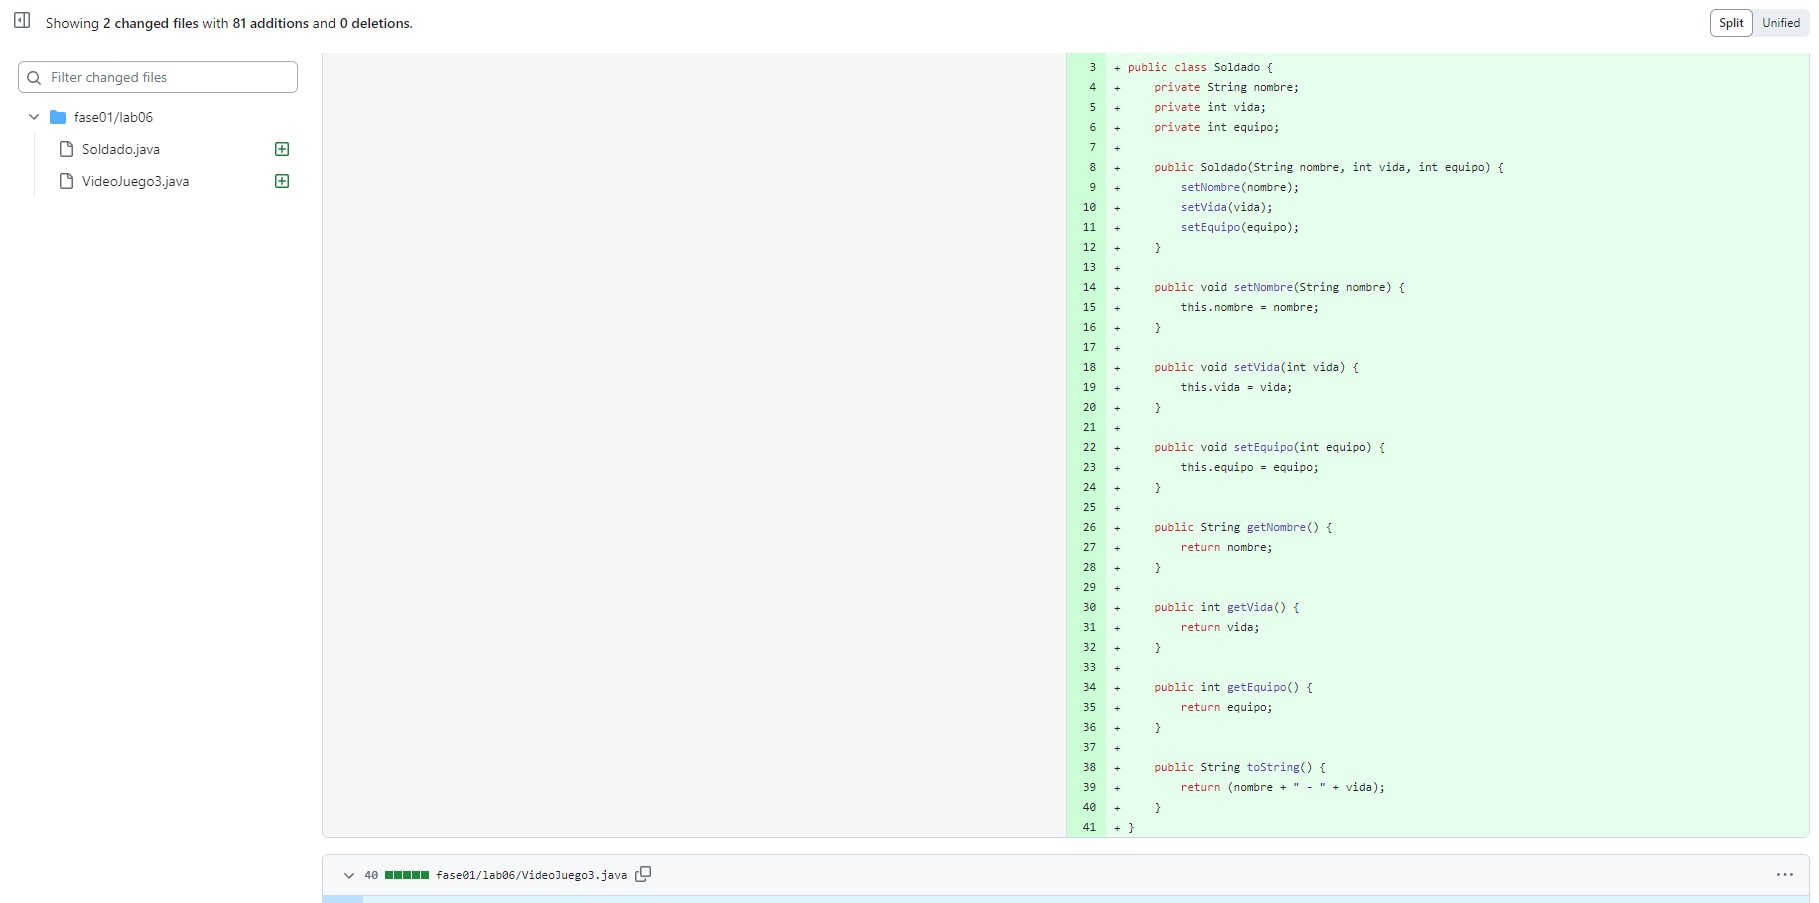
\includegraphics[width=1\textwidth,keepaspectratio]{img/commit01.jpg}
	\caption{Primer Commit.}
\end{figure}
\begin{lstlisting}[language=bash,caption={Actualizando VideoJuego3.java}]
		$ code VideoJuego3.java
	\end{lstlisting}
\begin{lstlisting}[language=bash,caption={Segundo - Decimo Segundo Commit / VideoJuego3.java}]
		$ git add VideoJuego3.java
		$ git commit -m "Metodo inicializarTablero()"
		$ code VideoJuego3.java
		$ git add VideoJuego3.java
		$ git commit -m "Metodo inicializarSoldados()"
		$ code VideoJuego3.java
		$ git add VideoJuego3.java
		$ git commit -m "Metodo imprimirTablero() y auxiliares"
		$ code VideoJuego3.java
		$ git add VideoJuego3.java
		$ git commit -m "Metodo soldadoMayorVida()"
		$ code VideoJuego3.java
		$ git add VideoJuego3.java
		$ git commit -m "Metodo promedioPuntosVida()"
		$ code VideoJuego3.java
		$ git add VideoJuego3.java
		$ git commit -m "Metodo imprimirSoldados()"
		$ code VideoJuego3.java
		$ git add VideoJuego3.java
		$ git commit -m "Metodo copiarArrayList()"
		$ code VideoJuego3.java
		$ git add VideoJuego3.java
		$ git commit -m "Metodo ordenarSoldadosBurbuja() y auxiliares"
		$ code VideoJuego3.java
		$ git add VideoJuego3.java
		$ git commit -m "Metodo ordenarSoldadosSeleccion()"
		$ code VideoJuego3.java
		$ git add VideoJuego3.java
		$ git commit -m "Metodo obtenerGanador() y auxiliares"
		$ code VideoJuego3.java
		$ git add VideoJuego3.java
		$ git commit -m "Correccion obtenerGanador() por imprimirGanador()"
		$ git push
	\end{lstlisting}
\begin{figure}[H]
	\centering
	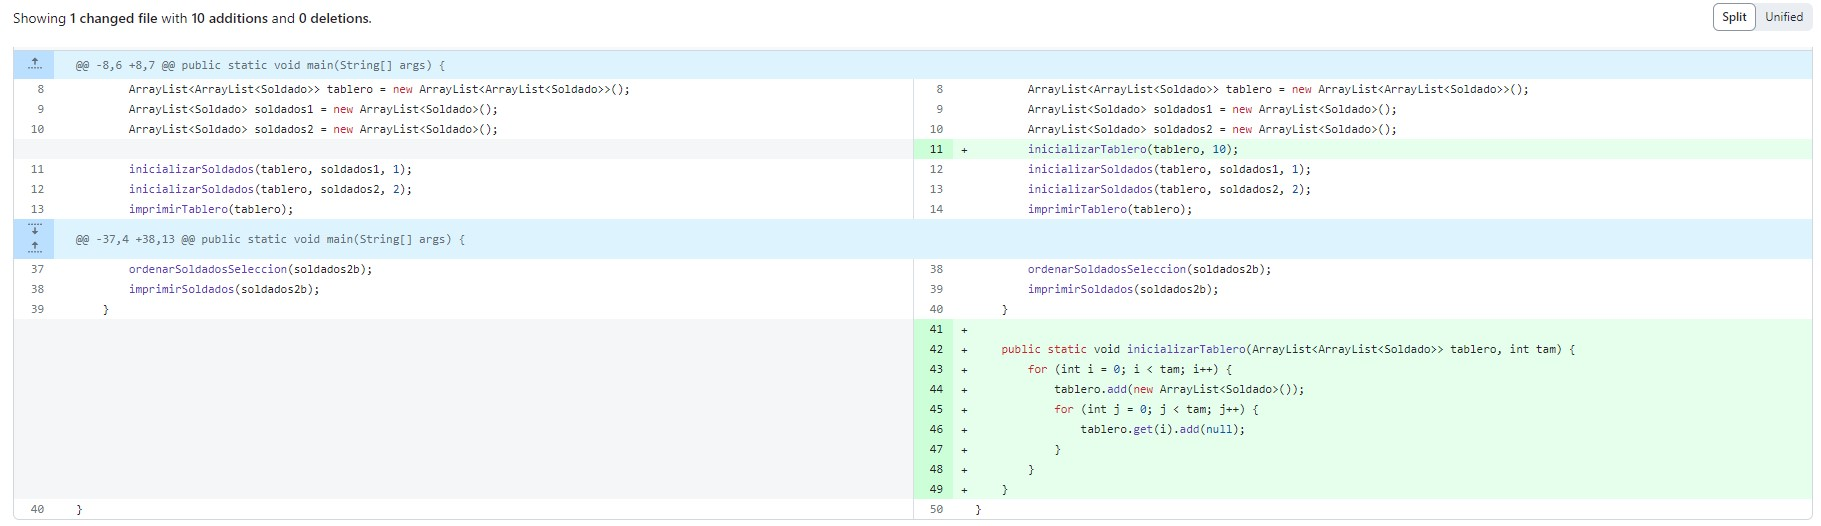
\includegraphics[width=1\textwidth,keepaspectratio]{img/commit02.jpg}
	\caption{Segundo Commit.}
\end{figure}
\begin{figure}[H]
	\centering
	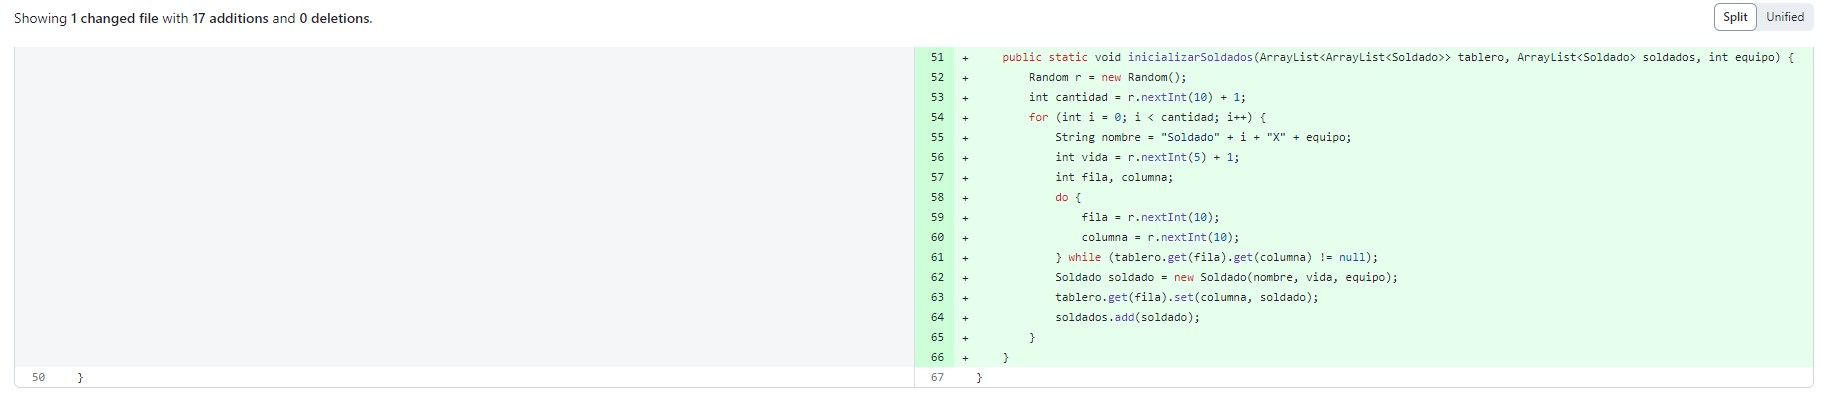
\includegraphics[width=1\textwidth,keepaspectratio]{img/commit03.jpg}
	\caption{Tercer Commit.}
\end{figure}
\begin{figure}[H]
	\centering
	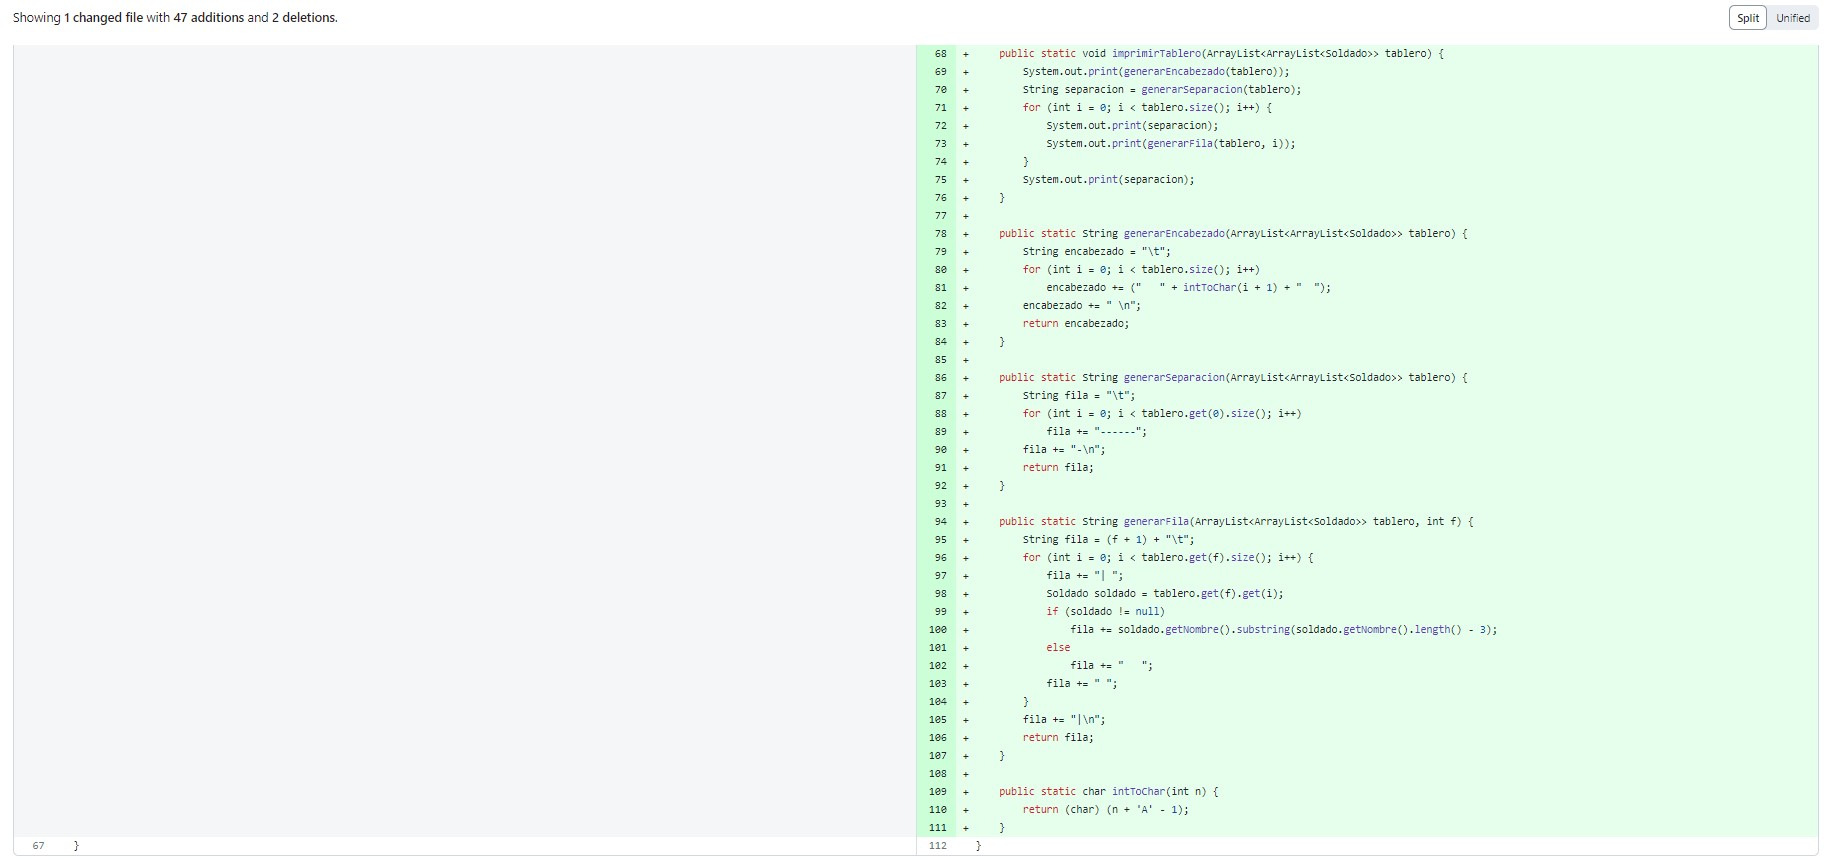
\includegraphics[width=1\textwidth,keepaspectratio]{img/commit04.jpg}
	\caption{Cuarto Commit.}
\end{figure}
\begin{figure}[H]
	\centering
	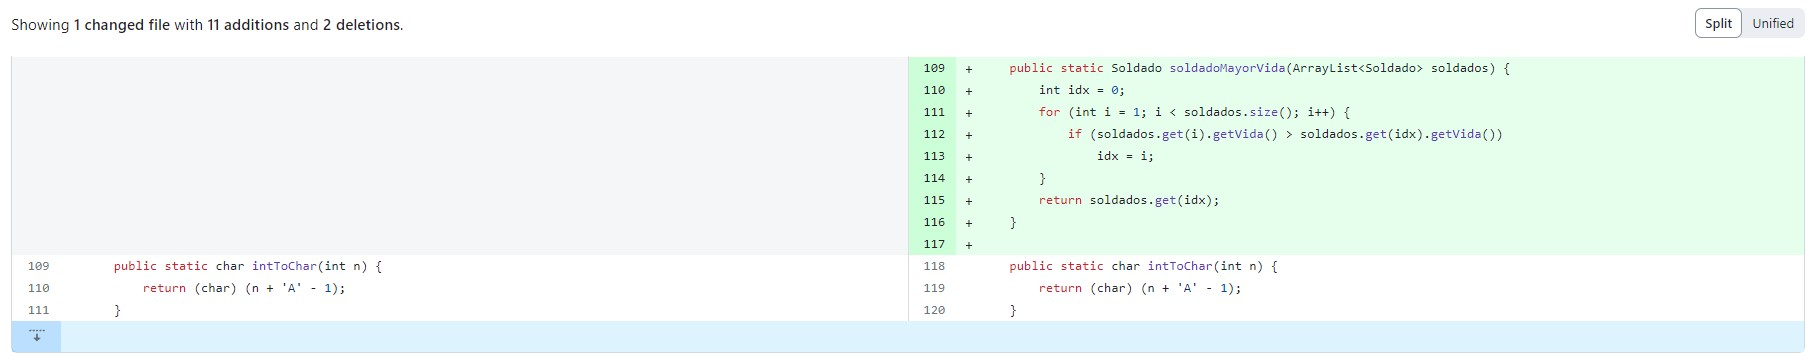
\includegraphics[width=1\textwidth,keepaspectratio]{img/commit05.jpg}
	\caption{Quinto Commit.}
\end{figure}
\begin{figure}[H]
	\centering
	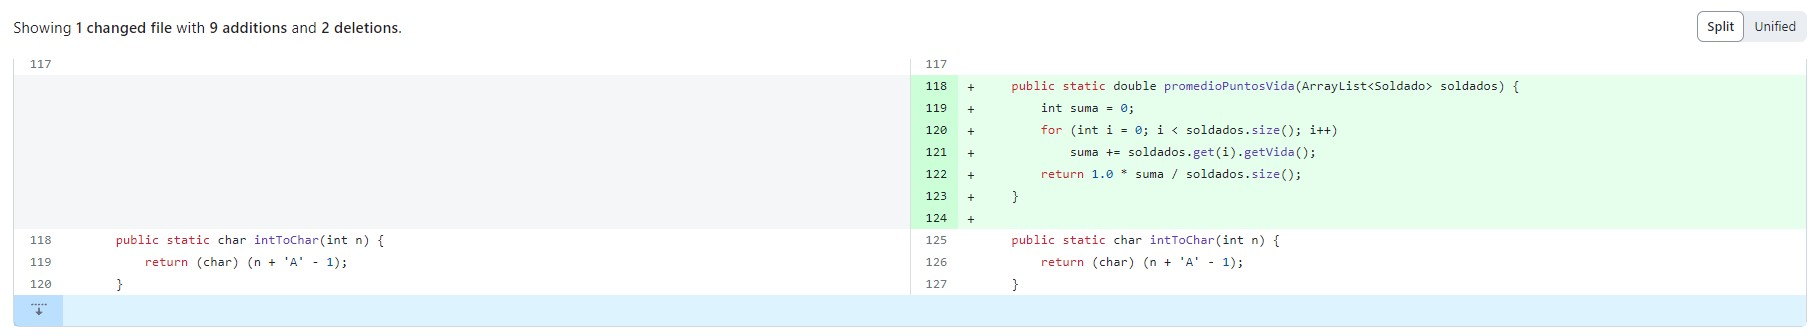
\includegraphics[width=1\textwidth,keepaspectratio]{img/commit06.jpg}
	\caption{Sexto Commit.}
\end{figure}
\begin{figure}[H]
	\centering
	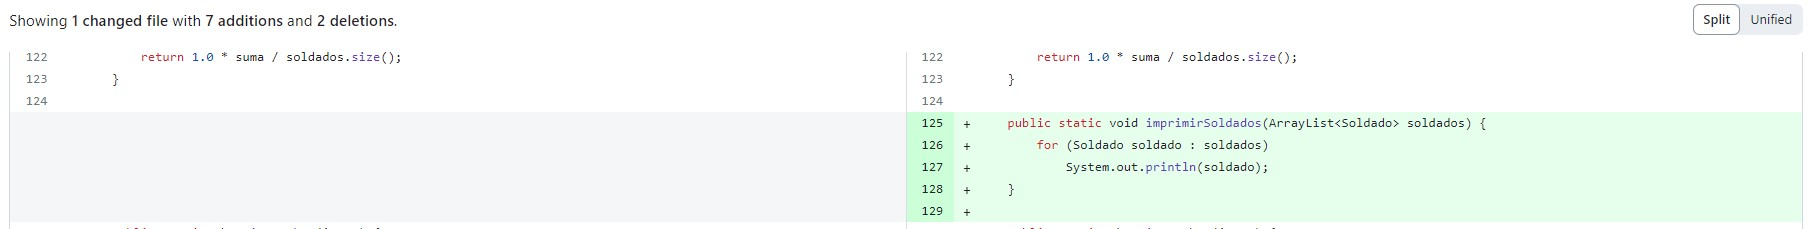
\includegraphics[width=1\textwidth,keepaspectratio]{img/commit07.jpg}
	\caption{Séptimo Commit.}
\end{figure}
\begin{figure}[H]
	\centering
	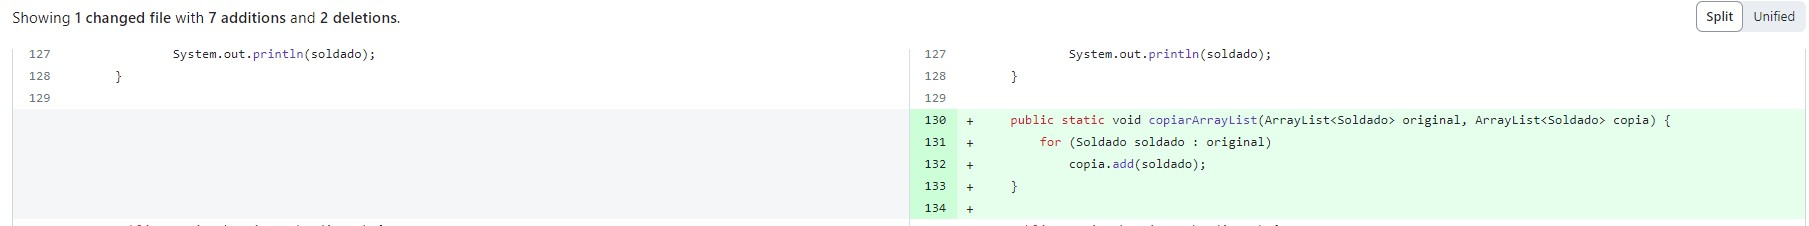
\includegraphics[width=1\textwidth,keepaspectratio]{img/commit08.jpg}
	\caption{Octavo Commit.}
\end{figure}
\begin{figure}[H]
	\centering
	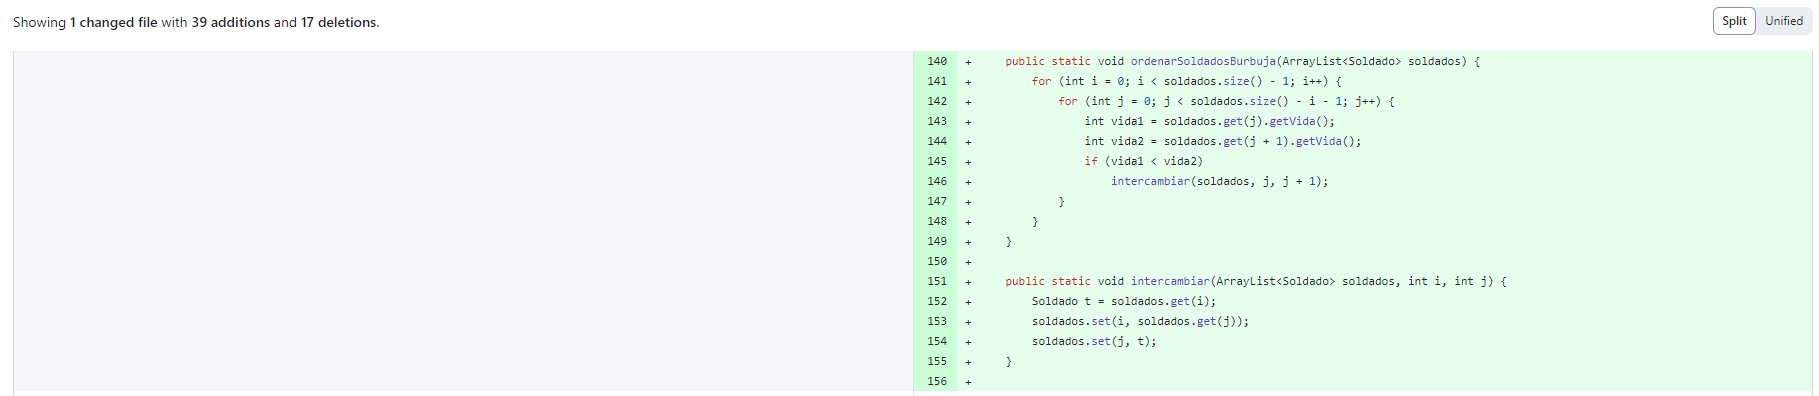
\includegraphics[width=1\textwidth,keepaspectratio]{img/commit09.jpg}
	\caption{Noveno Commit.}
\end{figure}
\begin{figure}[H]
	\centering
	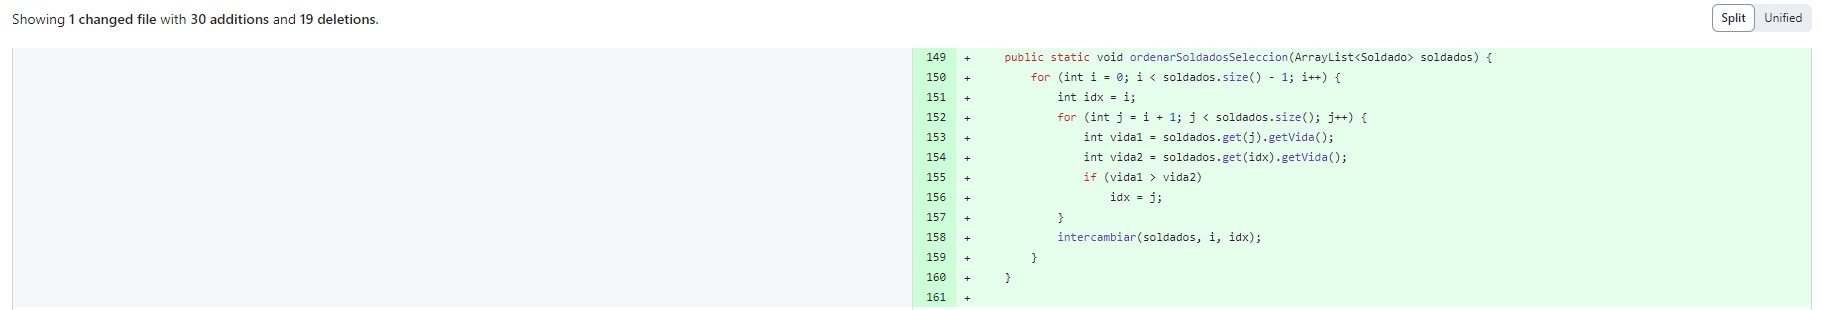
\includegraphics[width=1\textwidth,keepaspectratio]{img/commit10.jpg}
	\caption{Decimo Commit.}
\end{figure}
\begin{figure}[H]
	\centering
	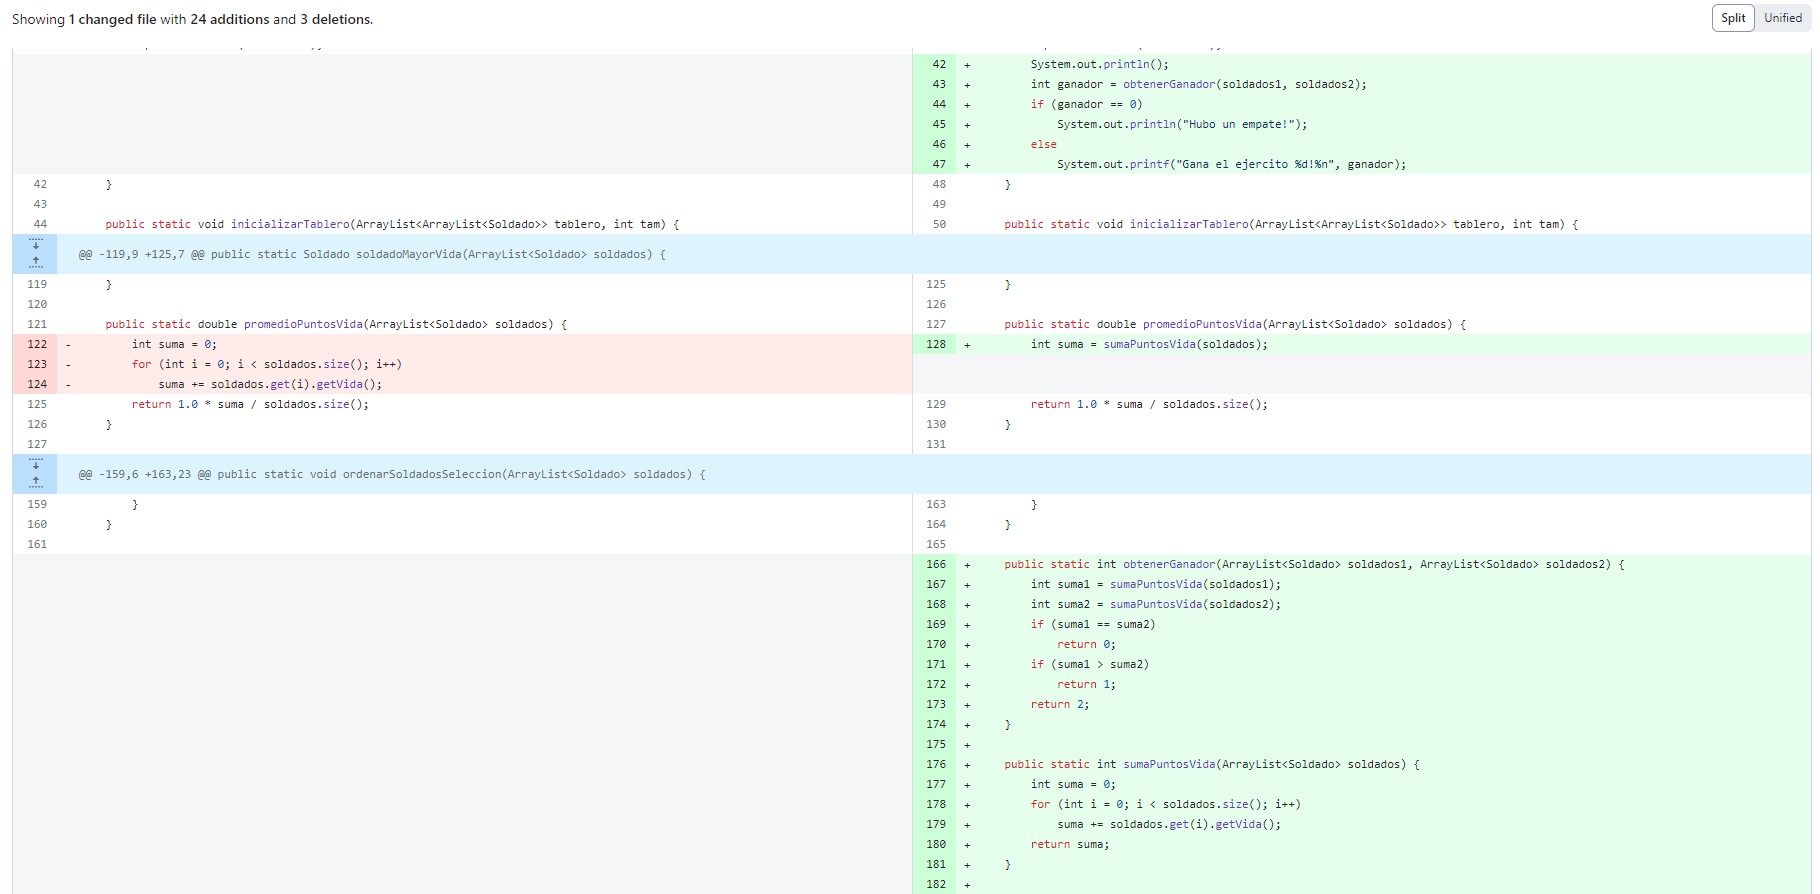
\includegraphics[width=1\textwidth,keepaspectratio]{img/commit11.jpg}
	\caption{Decimo Primer Commit.}
\end{figure}
\begin{figure}[H]
	\centering
	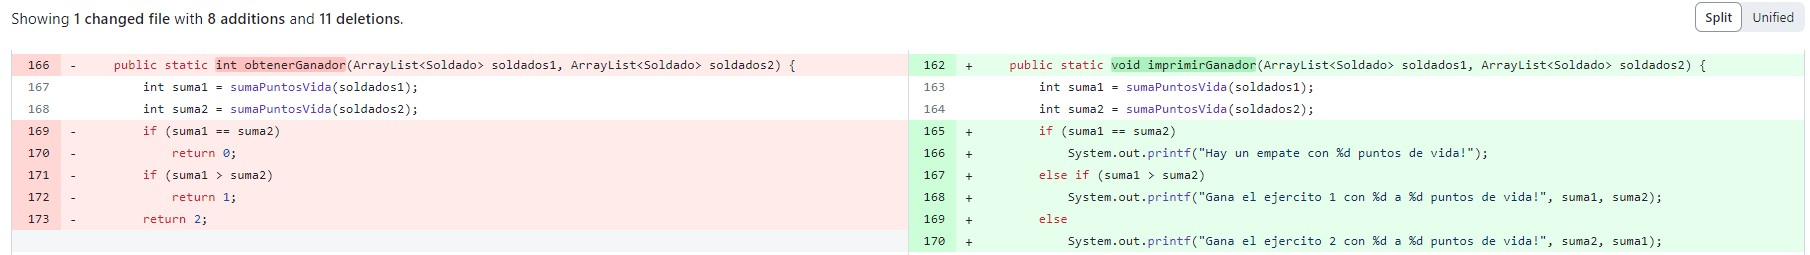
\includegraphics[width=1\textwidth,keepaspectratio]{img/commit12.jpg}
	\caption{Decimo Segundo Commit.}
\end{figure}
\pagebreak

\section{Código desarrollado}
\lstinputlisting[language=Java, caption={Soldado.java},numbers=left,]{Soldado.java}
\begin{itemize}
	\item Clase que guarda nombre y vida del soldado.
	\item Posee tanto setters como getters para todos los atributos.
	\item Posee el metodo toString() para poder imprimir el objeto.
\end{itemize}
\pagebreak
\lstinputlisting[language=Java, caption={VideoJuego3.java},numbers=left,]{VideoJuego3.java}
\begin{itemize}
	\item Método inicializarTablero() crea un tablero de 10x10 completamente vacio.
	\item Método inicializarSoldados() crea a los soldados, los ubica en el tablero y los guarda en un arreglo de soldados por separado.
	\item Método imprimirTablero() imprime el tablero con ayuda de los métodos auxiliares generarEncabezado(), generarSeparacion() y generarFila(), ubicando a los soldados por su numero.
	\item Método soldadoMayorVida() retorna el soldado con mayor vida.
	\item Método promedioPuntosVida() retorna el promedio de los puntos de vida de todos los soldados.
	\item Método imprimirSoldados() imprime los soldados del ejército.
	\item Se crean dos copias del arreglo de soldados para demostrar los 2 ordenamientos.
	\item Método ordenarSoldadosBurbuja() ordena los soldados por vida de mayor a menor, usando ordenamiento burbuja.
	\item Método ordenarSoldadosSeleccion() ordena los soldados por vida de mayor a menor, usando ordenamiento selección.
	\item Se reusan los métodos para mostrar los datos de ambos ejércitos.
	\item Método imprimirGanador() imprime el ejército ganador de acuerdo a la cantidad total de puntos de vida de cada uno.
\end{itemize}
\pagebreak

\section{Ejecución del código}
\lstinputlisting[keepspaces=true,language=bash,caption={VideoJuego3.java},numbers=left,]{ejec01.bash}
\pagebreak

\section{Estructura de laboratorio \itemPracticeNumber}
\begin{itemize}
	\item El contenido que se entrega en este laboratorio es el siguiente:
\end{itemize}
%%%%%%%%%%%%%%%%%%%%%%%%%%%%%%%%%%%%%%%%%%%%%%%%%%%%%%%%%%%%%%%%%%%%%%
\begin{lstlisting}[style=ascii-tree]
lab06/
|--- Soldado.java
|--- VideoJuego3.java
|--- ejec01.bash
|--- Informe.tex
|--- Informe.pdf
|--- img
	|--- logo_abet.png
	|--- logo_episunsa.png
	|--- logo_unsa.jpg
	|--- commit01.jpg
	|--- commit02.jpg
	|--- commit03.jpg
	|--- commit04.jpg
	|--- commit05.jpg
	|--- commit06.jpg
	|--- commit07.jpg
	|--- commit08.jpg
	|--- commit09.jpg
	|--- commit10.jpg
	|--- commit11.jpg
	|--- commit12.jpg
\end{lstlisting}
%%%%%%%%%%%%%%%%%%%%%%%%%%%%%%%%%%%%%%%%%%%%%%%%%%%%%%%%%%%%%%%%%%%%%%
\pagebreak

\section{\textcolor{red}{Rúbricas}}

\subsection{\textcolor{red}{Entregable Informe}}
\begin{table}[H]
	\caption{Tipo de Informe}
	\setlength{\tabcolsep}{0.5em} % for the horizontal padding
	{\renewcommand{\arraystretch}{1.5}% for the vertical padding
		\begin{tabular}{|M{3cm}|M{12cm}|}
			\hline
			\multicolumn{2}{|c|}{\textbf{\textcolor{red}{Informe}}}                                                                                                      \\
			\hline
			\textbf{\textcolor{red}{Latex}} & \textcolor{blue}{El informe está en formato PDF desde Latex,  con un formato limpio (buena presentación) y facil de leer.} \\
			\hline
		\end{tabular}
	}
\end{table}

\subsection{\textcolor{red}{Rúbrica para el contenido del Informe y demostración}}
\begin{itemize}
	\item El alumno debe marcar o dejar en blanco en celdas de la columna \textbf{Checklist} si cumplio con el ítem correspondiente.
	\item Si un alumno supera la fecha de entrega, su calificación será sobre la nota mínima aprobatoria, siempre y cuando cumpla con todos los items.
	\item El alumno debe autocalificarse en la columna \textbf{Estudiante} de acuerdo a la siguiente tabla:

	      \begin{table}[ht]
		      \caption{Niveles de desempeño}
		      \begin{center}
			      \begin{tabular}{ccccc}
				      \hline
				                      & \multicolumn{4}{c}{Nivel}                                                              \\
				      \cline{1-5}
				      \textbf{Puntos} & Insatisfactorio 25\%      & En Proceso 50\% & Satisfactorio 75\% & Sobresaliente 100\% \\
				      \textbf{2.0}    & 0.5                       & 1.0             & 1.5                & 2.0                 \\
				      \textbf{4.0}    & 1.0                       & 2.0             & 3.0                & 4.0                 \\
				      \hline
			      \end{tabular}
		      \end{center}
	      \end{table}

\end{itemize}

\begin{table}[H]
	\caption{Rúbrica para contenido del Informe y demostración}
	\setlength{\tabcolsep}{0.5em} % for the horizontal padding
	{\renewcommand{\arraystretch}{1.5}% for the vertical padding
		%\begin{center}
		\begin{tabular}{|M{2.3cm}|M{5cm}|M{1.2cm}|M{1.5cm}|M{1.8cm}|M{1.4cm}|}
			\hline
			\multicolumn{2}{|c|}{Contenido y demostración} & Puntos                                                                                                                                                                                                          & Checklist & Estudiante & Profesor   \\
			\hline
			\textbf{1. GitHub}                             & Hay enlace URL activo del directorio para el  laboratorio hacia su repositorio GitHub con código fuente terminado y fácil de revisar.                                                                           & 2         & X          & 2        & \\
			\hline
			\textbf{2. Commits}                            & Hay capturas de pantalla de los commits más importantes con sus explicaciones detalladas. (El profesor puede preguntar para refrendar calificación).                                                            & 4         & X          & 3        & \\
			\hline
			\textbf{3. Código fuente}                      & Hay porciones de código fuente importantes con numeración y explicaciones detalladas de sus funciones.                                                                                                          & 2         & X          & 2        & \\
			\hline
			\textbf{4. Ejecución}                          & Se incluyen ejecuciones/pruebas del código fuente explicadas gradualmente.                                                                                                                                      & 2         & X          & 1.5      & \\
			\hline
			\textbf{5. Pregunta}                           & Se responde con completitud a la pregunta formulada en la tarea.  (El profesor puede preguntar para refrendar calificación).                                                                                    & 2         & X          & 2        & \\
			\hline
			\textbf{6. Fechas}                             & Las fechas de modificación del código fuente estan dentro de los plazos de fecha de entrega establecidos.                                                                                                       & 2         & X          & 2        & \\
			\hline
			\textbf{7. Ortografía}                         & El documento no muestra errores ortográficos.                                                                                                                                                                   & 2         & X          & 1.5      & \\
			\hline
			\textbf{8. Madurez}                            & El Informe muestra de manera general una evolución de la madurez del código fuente,  explicaciones puntuales pero precisas y un acabado impecable.   (El profesor puede preguntar para refrendar calificación). & 4         & X          & 4        & \\
			\hline
			\multicolumn{2}{|c|}{\textbf{Total}}           & 20                                                                                                                                                                                                              &           & 18         &            \\
			\hline
		\end{tabular}
		%\end{center}
		%\label{tab:multicol}
	}
\end{table}

\section{Referencias}
\begin{itemize}
	\item Aedo, M. y Castro, E. (2021). FUNDAMENTOS DE PROGRAMACIÓN 2 - Tópicos de Programación Orientada a Objetos. Editorial UNSA.
\end{itemize}

%\pagebreak
%\bibliographystyle{apalike}
%\bibliographystyle{IEEEtranN}
%\bibliography{bibliography}

\end{document}